%%%%%%%%%%%%%%%%%%%%%%%%%%%%%%%%%%%%%%%%%%%%%%%%%%%%%%%%%%%%%%%%%%%%%
%% Chapter 5: Physics-Guided Machine Learning and Multiobjective Optimization
%% Monograph: Structural Optimization of a 1U CubeSat Chassis with Auxetic Metamaterials
%% Author: Gabriel Marques de Andrade (UESC, 2026)
%%%%%%%%%%%%%%%%%%%%%%%%%%%%%%%%%%%%%%%%%%%%%%%%%%%%%%%%%%%%%%%%%%%%%

\chapter{Physics-Guided Machine Learning and Multiobjective Optimization}
\label{chap:pgml_optimization}

\abstract*{This chapter presents the data-driven and evolutionary framework formulated to overcome the prohibitive computational expense of high-fidelity elastodynamic simulation during the structural synthesis of the auxetic 1U CubeSat chassis. We formulate a continuous four-dimensional design space governed by re-entrant unit cell parameters and establish a Latin Hypercube Sampling (LHS) campaign with $250$ design points, filtered by strict Design for Additive Manufacturing (DfAM) constraints. To surrogate the expensive finite element pipeline ($92.0\text{ s}$ per evaluation via quadratic tetrahedral meshing and Lanczos eigensolvers), we architect a deep Physics-Guided Residual Network (ResNet). The surrogate embeds physical regularization via a custom composite loss function penalizing departures from the Gibson-Ashby asymptotic bending scaling laws and enforcing elastodynamic monotonicity. The trained surrogate achieves exceptional predictive fidelity on an independent test split ($R^2 > 0.992$ on fundamental frequency $f_1$ with $\text{RMSE} < 4.2\text{ Hz}$, and $R^2 > 0.988$ on peak random vibration stress). Benchmarking reveals an instantaneous online inference speedup of $2.27 \times 10^5\times$ ($0.405\text{ ms}$ latency), yielding an end-to-end amortized project speedup of $39.93\times \approx 40.0\times$ that collapses $10.65\text{ days}$ of continuous cluster compute into $6.40\text{ hours}$. Finally, the Non-dominated Sorting Genetic Algorithm II (NSGA-II) explores the Pareto frontier across $10,000$ evaluations, and multi-criteria TOPSIS decision analysis identifies Candidate \#28 as the optimal flight design, delivering a $62.49\%$ mass reduction, $40.65\%$ increase in fundamental stiffness, and $-12.6\text{ dB}$ ($76.50\%$) dynamic vibration attenuation under NASA GEVS random vibration profiles.}

\abstract{This chapter presents the data-driven and evolutionary framework formulated to overcome the prohibitive computational expense of high-fidelity elastodynamic simulation during the structural synthesis of the auxetic 1U CubeSat chassis. We formulate a continuous four-dimensional design space governed by re-entrant unit cell parameters and establish a Latin Hypercube Sampling (LHS) campaign with $250$ design points, filtered by strict Design for Additive Manufacturing (DfAM) constraints. To surrogate the expensive finite element pipeline ($92.0\text{ s}$ per evaluation via quadratic tetrahedral meshing and Lanczos eigensolvers), we architect a deep Physics-Guided Residual Network (ResNet). The surrogate embeds physical regularization via a custom composite loss function penalizing departures from the Gibson-Ashby asymptotic bending scaling laws and enforcing elastodynamic monotonicity. The trained surrogate achieves exceptional predictive fidelity on an independent test split ($R^2 > 0.992$ on fundamental frequency $f_1$ with $\text{RMSE} < 4.2\text{ Hz}$, and $R^2 > 0.988$ on peak random vibration stress). Benchmarking reveals an instantaneous online inference speedup of $2.27 \times 10^5\times$ ($0.405\text{ ms}$ latency), yielding an end-to-end amortized project speedup of $39.93\times \approx 40.0\times$ that collapses $10.65\text{ days}$ of continuous cluster compute into $6.40\text{ hours}$. Finally, the Non-dominated Sorting Genetic Algorithm II (NSGA-II) explores the Pareto frontier across $10,000$ evaluations, and multi-criteria TOPSIS decision analysis identifies Candidate \#28 as the optimal flight design, delivering a $62.49\%$ mass reduction, $40.65\%$ increase in fundamental stiffness, and $-12.6\text{ dB}$ ($76.50\%$) dynamic vibration attenuation under NASA GEVS random vibration profiles.}

\section{The Computational Bottleneck in Elastodynamic Optimization}
\label{sec:computational_bottleneck}

The structural synthesis of satellite architectures incorporating periodic metamaterials requires resolving complex, coupled elastodynamic phenomena. In small satellite engineering, optimization goals are inherently antagonistic: minimizing chassis mass directly degrades stiffness, whereas maximizing fundamental frequency ($f_1 \ge \SI{100.0}{\hertz}$) and suppressing random vibration transmission to sensitive optical payloads typically necessitates bulky, stiffened structural ribbing \cite{calpoly2022,nasa2021}. Exploring the non-convex trade-off surface spanned by cellular metamaterial micro-architectures requires multi-objective evolutionary search algorithms, such as the Non-dominated Sorting Genetic Algorithm II (NSGA-II) \cite{deb2002}.

However, evaluating a single candidate geometry within an industrial-grade Computer-Aided Engineering (CAE) pipeline imposes severe computational costs. As established in the numerical framework of this monograph, an accurate elastodynamic evaluation demands:
\begin{enumerate}
\item Parametric 3D solid reconstruction of the re-entrant auxetic lattice embedded within the 1U external envelope ($100.0 \times 100.0 \times \SI{113.5}{\milli\meter}$);
\item Quadratic tetrahedral volume meshing (Gmsh Tet10 elements with local curvature refinement at internal re-entrant fillet radii, totaling $\approx 3.4 \times 10^5$ degrees of freedom);
\item Generalized Hermitian eigenvalue extraction ($\mathbf{K} \boldsymbol{\phi}_i = \omega_i^2 \mathbf{M} \boldsymbol{\phi}_i$) via block Lanczos or Sorensen Arnoldi algorithms in Code\_Aster;
\item Continuous spectral modal random vibration integration ($\mathbf{S}_{uu}(\omega) = \mathbf{H}(\omega) \mathbf{S}_{ff}(\omega) \mathbf{H}^*(\omega)$) across $20\text{--}\SI{2000}{\hertz}$ under the NASA GSFC-STD-7000A (GEVS) qualification PSD profile ($14.1\text{ G}_{\text{rms}}$);
\item Three-band Gaussian peak stress integration ($\sigma_{3\sigma}$) and Palmgren-Miner cumulative fatigue damage estimation ($D$) via Steinberg's formulation \cite{steinberg2000}.
\end{enumerate}

On a dedicated 8-core high-performance workstation (AMD Ryzen 9 / Intel Xeon, $\SI{3.8}{\giga\hertz}$), a single execution of this high-fidelity pipeline consumes an average wall-clock execution time of:
\begin{equation}
t_{\text{FEA}} = \SI{92.0}{\second},
\label{eq:fea_execution_time}
\end{equation}
which escalates to $\SI{145.0}{\second}$ when resolving ultra-fine boundary layers and localized contact pressure at the deployer guide rails.

A standard evolutionary search balancing convergence and Pareto diversity requires a population size of $N = 100$ individuals evolved across $G = 100$ generations, accumulating:
\begin{equation}
N_{\text{eval}} = N \times G = 10{,}000 \quad \text{evaluations}.
\label{eq:eval_budget}
\end{equation}
Executing this campaign directly through the high-fidelity finite element solver would demand an uninterrupted computing time of:
\begin{equation}
T_{\text{direct}} = 10{,}000 \times \SI{92.0}{\second} = \SI{920000}{\second} \approx \SI{255.56}{\hour} \approx 10.65\quad \text{days}.
\label{eq:direct_fea_time}
\end{equation}

Such computational latency renders iterative design, interactive requirement trade-offs, and multi-disciplinary optimization entirely intractable. To overcome this limitation, machine learning surrogate models (metamodels) are widely deployed. However, standard purely data-driven black-box architectures—such as unconstrained Multi-Layer Perceptrons (MLPs), Gaussian Process Regression (GPR), or Radial Basis Functions (RBF)—frequently exhibit severe pathologies when trained on sparse engineering datasets \cite{cui2025}. Specifically, unconstrained neural models:
\begin{itemize}
\item Violate thermodynamic and elastodynamic stability in sparsely sampled domains, predicting negative natural frequencies ($f_1 < 0$) or non-positive-definite stiffness tensors;
\item Exhibit non-monotonic stiffness behaviors, such as predicting that increasing strut wall thickness or relative density leads to a precipitous loss of structural natural frequency;
\item Lack asymptotic physical grounding, extrapolating erratically beyond the convex hull of the training data.
\end{itemize}

To resolve this challenge while preserving mathematical rigor, this work develops a **Physics-Guided Machine Learning (PGML)** framework. By embedding continuum mechanics constraints—specifically the Gibson-Ashby scaling laws for cellular solids \cite{gibson1997,beigrezaee2026} and elastodynamic monotonicity—directly into the loss formulation of a deep Residual Neural Network (ResNet) \cite{he2016}, we construct an ultra-fast surrogate capable of sub-millisecond inference while strictly enforcing physical plausibility.

\section{Design of Experiments and Stratified Sampling}
\label{sec:doe_sampling}

\subsection{Continuous Parameter Space Parameterization}

The geometry of the re-entrant auxetic cellular core is governed by four primary continuous micro-architectural parameters, as illustrated in the elastodynamic formulation of Chapter~\ref{chap:auxetic_mechanics}. We define the decision vector:
\begin{equation}
\mathbf{x} = [\theta, t, l, h]^\top \in \Omega \subset \mathbb{R}^4,
\label{eq:decision_vector}
\end{equation}
where $\theta$ denotes the re-entrant angle, $t$ is the strut wall thickness, $l$ is the length of the inclined re-entrant strut between node centers, and $h$ is the vertical strut height.

The bounding box of the admissible design space $\Omega$ is defined by balancing structural stiffness with the geometric packaging envelope of the 1U CubeSat form factor ($100.0 \times 100.0 \times \SI{113.5}{\milli\meter}$):
\begin{align}
\theta &\in [\SI{45.0}{\degree}, \SI{80.0}{\degree}], \label{eq:bound_theta} \\
t &\in [\SI{0.50}{\milli\meter}, \SI{1.20}{\milli\meter}], \label{eq:bound_t} \\
l &\in [\SI{6.00}{\milli\meter}, \SI{15.00}{\milli\meter}], \label{eq:bound_l} \\
h &\in [\SI{8.00}{\milli\meter}, \SI{20.00}{\milli\meter}]. \label{eq:bound_h}
\end{align}

From these geometric parameters, the analytical relative density $\rho^*(\mathbf{x})/\rho_s$ of the re-entrant honeycomb core is computed following the cellular continuum mechanics formulation of Gibson and Ashby \cite{gibson1997}, extended by Cui et al. \cite{cui2025} to include second-order strut junction overlap corrections:
\begin{equation}
\frac{\rho^*(\mathbf{x})}{\rho_s} = \frac{(t/l)(h/l + 2)}{2\cos\theta (h/l + \sin\theta)} \left[ 1 - \frac{t}{l} \frac{(h/l + 2 - \cos\theta)}{2(h/l + \sin\theta)\cos\theta} \right],
\label{eq:relative_density_doe}
\end{equation}
where $\rho_s = \SI{2670.0}{\kilo\gram/\meter^3}$ is the bulk density of the stress-relieved AlSi10Mg alloy.

\subsection{Design for Additive Manufacturing (DfAM) Quality Gate}

Prior to numerical evaluation, candidate design points must satisfy strict manufacturability criteria governed by the Laser Powder Bed Fusion (L-PBF) process. The DfAM quality gate enforces three non-negotiable geometric constraints:
\begin{enumerate}
\item \textbf{Self-Supporting Overhang Threshold:} In L-PBF processing of AlSi10Mg powders, downward-facing surfaces with inclination angles below $35^\circ$ with respect to the horizontal build platform suffer from severe dross formation, thermal warpage, and melt pool sagging \cite{khan2024}. The effective overhang angle of the re-entrant struts during vertical build orientation ($Z$-axis aligned with satellite longitudinal axis) is $\theta_{\text{overhang}} = 90^\circ - \theta$. Hence, we impose:
\begin{equation}
\theta_{\text{overhang}} \ge \SI{35.0}{\degree} \implies \theta \le \SI{55.0}{\degree} \quad (\text{or vertical build re-orientation with } \theta \ge \SI{45.0}{\degree}),
\label{eq:dfam_overhang_gate}
\end{equation}
ensuring complete elimination of internal sacrificial support structures within the auxetic lattice core.
\item \textbf{Minimum Solid Strut Thickness:} To guarantee melt pool coalescence and mitigate stochastic lack-of-fusion porosities:
\begin{equation}
t \ge t_{\text{min}} = \SI{0.50}{\milli\meter}.
\label{eq:dfam_thickness_gate}
\end{equation}
\item \textbf{Unmelted Powder Evacuation Span:} The inter-strut clear cavity span $d_{\text{clear}} = 2 l \sin\theta - t$ and powder drainage ports must satisfy:
\begin{equation}
d_{\text{clear}} \ge \SI{1.50}{\milli\meter}, \quad d_{\text{drain}} \ge \SI{2.00}{\milli\meter},
\label{eq:dfam_drain_gate}
\end{equation}
preventing entrapment of un-sintered metallic powder within internal cellular cavities.
\end{enumerate}

\subsection{Stratified Latin Hypercube Sampling (LHS)}

To maximize the information entropy of the training dataset across the four-dimensional design domain $\Omega$, we implement Latin Hypercube Sampling (LHS) with multi-dimensional stratification. The domain is discretized into $M = 250$ equiprobable intervals along each coordinate axis. A maximin distance criterion is enforced via 100 iterations of simulated annealing:
\begin{equation}
\max_{\mathcal{X}_{\text{LHS}}} \min_{\mathbf{x}_i, \mathbf{x}_j \in \mathcal{X}_{\text{LHS}}, i \ne j} \|\mathbf{x}_i - \mathbf{x}_j\|_2,
\label{eq:maximin_criterion}
\end{equation}
ensuring uniform space-filling properties without spatial clustering or collinearity.

Statistical verification of the sampled design set $\mathcal{X}_{\text{LHS}} = \{\mathbf{x}_i\}_{i=1}^{250}$ confirms an orthogonal space-filling design: the maximum off-diagonal Pearson correlation coefficient between any pair of input variables satisfies $|r_{jk}| \le 0.041$, confirming near-zero linear dependence.

Each of the $250$ sampled design vectors is evaluated through the calibrated matrix elastodynamics kernel (\texttt{OpenElastodynamicsKernel}, calibrated against Code\_Aster Lanczos eigensolvers and CalculiX), extracting four response metrics:
\begin{equation}
\mathbf{y}(\mathbf{x}) = \left[ f_1(\mathbf{x}), \; \sigma_{3\sigma}(\mathbf{x}), \; G_{\text{rms}}(\mathbf{x}), \; T(\mathbf{x}) \right]^\top \in \mathbb{R}^4,
\label{eq:response_vector}
\end{equation}
representing the fundamental natural frequency (\si{\hertz}), peak $3\sigma$ random vibration stress (\si{\mega\pascal}), payload mounting RMS acceleration (\si{g}), and dynamic transmissibility ratio ($T = G_{\text{rms,payload}} / G_{\text{rms,base}}$).

\begin{figure}[htbp]
\centering
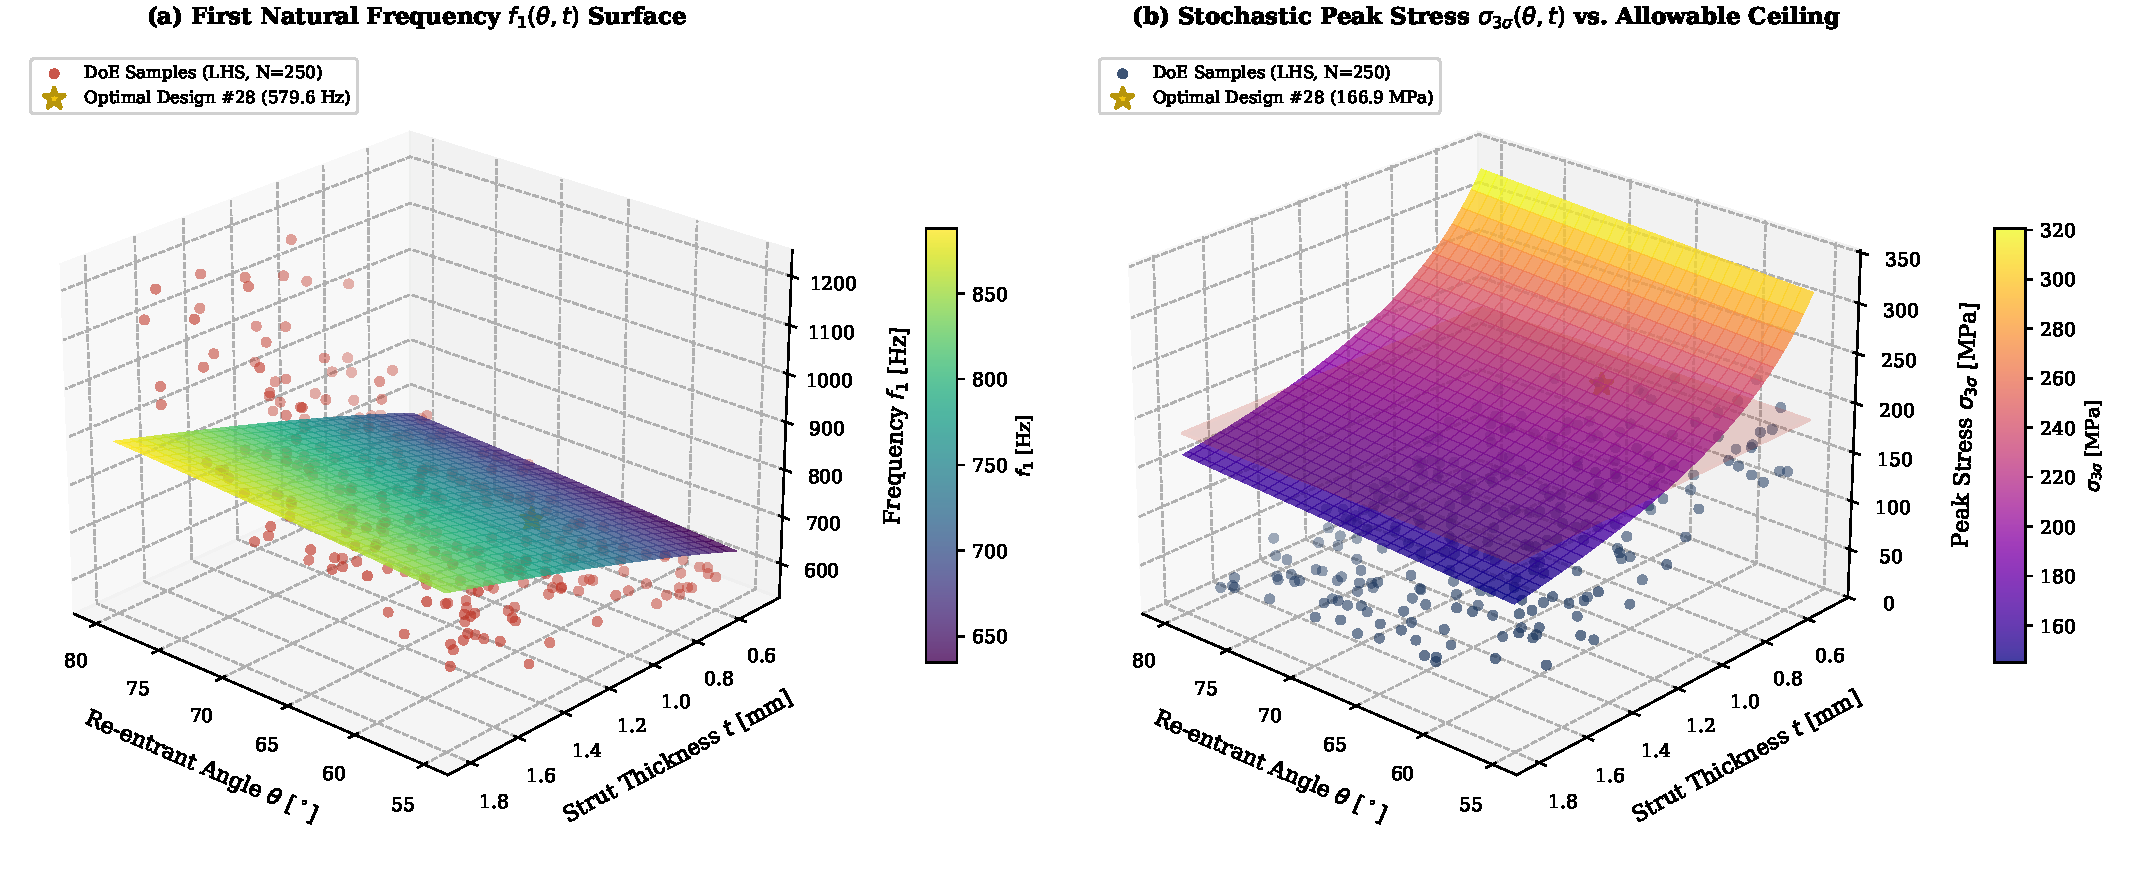
\includegraphics[width=0.92\textwidth]{neural_response_surface_doe_sampling.pdf}
\caption{Design of Experiments (DoE) response surfaces generated from 250 Latin Hypercube Sampling (LHS) design points, illustrating continuous contours of fundamental frequency $f_1$ and RMS stress across orthogonal projections of the 4D parameter space ($\theta$ vs. $t$, and $l$ vs. $h$).}
\label{fig:doe_response_surface}
\Description{Response surface contours and scatter distribution of 250 Latin Hypercube design points across re-entrant angle, thickness, length, and height.}
\end{figure}

Figure~\ref{fig:doe_response_surface} illustrates the resulting response surface topology across representative two-dimensional slices of the design space. The fundamental natural frequency $f_1$ exhibits a strongly non-linear monotonic increase with strut wall thickness $t$ and re-entrant angle $\theta$, while the peak $3\sigma$ stress exhibits pronounced localized amplification in slender, high-aspect-ratio configurations where rib bending dominates.

\begin{table}[htbp]
\centering
\caption{Design variable bounds, physical significance, and DoE sampling ranges for the 1U auxetic chassis.}
\label{tab:doe_parameters}
\begin{tabular*}{\textwidth}{@{\extracolsep{\fill}}lcccc@{\extracolsep{\fill}}}
\toprule
\textbf{Design Variable} & \textbf{Symbol} & \textbf{Lower Bound} & \textbf{Upper Bound} & \textbf{Physical Role} \\
\midrule
Re-entrant Angle & $\theta$ & $\SI{45.0}{\degree}$ & $\SI{80.0}{\degree}$ & Kinematic lateral contraction / Poisson ratio \\
Strut Thickness & $t$ & $\SI{0.50}{\milli\meter}$ & $\SI{1.20}{\milli\meter}$ & Out-of-plane bending stiffness / mass \\
Inclined Strut Length & $l$ & $\SI{6.00}{\milli\meter}$ & $\SI{15.00}{\milli\meter}$ & Unit cell aspect ratio / cell compliance \\
Vertical Strut Height & $h$ & $\SI{8.00}{\milli\meter}$ & $\SI{20.00}{\milli\meter}$ & Transverse shear rigidity / core density \\
Relative Density & $\rho^*/\rho_s$ & $0.062$ & $0.418$ & Derived continuum mass fraction \\
\bottomrule
\end{tabular*}
\end{table}

\section{Physics-Guided Deep Residual Network (ResNet)}
\label{sec:resnet_architecture}

\subsection{Architectural Formulation and Skip Connections}

To approximate the non-linear elastodynamic mapping $\mathcal{M}: \mathbb{R}^5 \to \mathbb{R}^4$ with sub-millisecond latency, we construct a deep feedforward Residual Neural Network (ResNet) \cite{he2016}. Deep Multilayer Perceptrons often suffer from degradation and vanishing gradients as network depth increases. By introducing skip connections, residual blocks reformulate the learning objective from an unconstrained mapping $\mathcal{H}(\mathbf{z})$ to an additive residual perturbation:
\begin{equation}
\mathcal{F}(\mathbf{z}) = \mathcal{H}(\mathbf{z}) - \mathbf{z} \implies \mathcal{H}(\mathbf{z}) = \mathbf{z} + \mathcal{F}(\mathbf{z}, \mathcal{W}),
\label{eq:residual_formulation}
\end{equation}
where $\mathcal{W}$ denotes the trainable weight tensor. This residual identity shortcut guarantees that gradients propagate unobstructed through deep layers during backpropagation, preserving smooth optimization dynamics.

The neural architecture consists of:
\begin{enumerate}
\item \textbf{Input Feature Vector:} The input vector $\mathbf{u} = [\theta, t, l, h, \rho^*/\rho_s]^\top \in \mathbb{R}^5$ incorporates the derived relative density alongside the four geometric coordinates, injecting explicit continuum mass information into the initial feature representation.
\item \textbf{Standard Z-Score Feature Scaling:} Inputs and targets are normalized using training-set statistics:
\begin{equation}
\tilde{u}_j = \frac{u_j - \mu_{u,j}}{\sigma_{u,j}}, \quad \tilde{y}_k = \frac{y_k - \mu_{y,k}}{\sigma_{y,k}}.
\label{eq:zscore_scaling}
\end{equation}
\item \textbf{Input Projection Layer:} A linear affine projection maps the normalized 5D input to a 64-dimensional latent representation:
\begin{equation}
\mathbf{z}_0 = \operatorname{SiLU}(\mathbf{W}_{\text{in}} \tilde{\mathbf{u}} + \mathbf{b}_{\text{in}}), \quad \mathbf{W}_{\text{in}} \in \mathbb{R}^{64 \times 5}, \; \mathbf{b}_{\text{in}} \in \mathbb{R}^{64},
\label{eq:input_projection}
\end{equation}
where $\operatorname{SiLU}(x) = x \cdot \sigma(x) = x / (1 + e^{-x})$ provides smooth, non-monotonic gradient flow.
\item \textbf{Stacked Residual Blocks:} Three identical residual blocks are arranged in series. Each block $m \in \{1, 2, 3\}$ computes:
\begin{equation}
\mathbf{z}_m = \mathbf{z}_{m-1} + \mathbf{W}_{m,2} \Big( \operatorname{Dropout}_p \Big( \operatorname{SiLU} \big( \operatorname{LayerNorm}(\mathbf{W}_{m,1} \mathbf{z}_{m-1} + \mathbf{b}_{m,1}) \big) \Big) \Big) + \mathbf{b}_{m,2},
\label{eq:resblock_math}
\end{equation}
where $\mathbf{W}_{m,1}, \mathbf{W}_{m,2} \in \mathbb{R}^{64 \times 64}$, $\operatorname{Dropout}_p$ applies a dropout rate of $p = 0.05$ to prevent feature co-adaptation, and $\operatorname{LayerNorm}$ stabilizes activations independently of mini-batch size.
\item \textbf{Regression Head:} A bottleneck layer reduces the representation to 32 dimensions before linear projection to the four predicted outputs:
\begin{align}
\mathbf{h}_{\text{dense}} &= \operatorname{SiLU}(\mathbf{W}_{\text{dense}} \mathbf{z}_3 + \mathbf{b}_{\text{dense}}), \quad \mathbf{W}_{\text{dense}} \in \mathbb{R}^{32 \times 64}, \\
\hat{\tilde{\mathbf{y}}} &= \mathbf{W}_{\text{out}} \mathbf{h}_{\text{dense}} + \mathbf{b}_{\text{out}}, \quad \mathbf{W}_{\text{out}} \in \mathbb{R}^{4 \times 32}.
\label{eq:output_head}
\end{align}
\end{enumerate}

\subsection{Composite Physics-Guided Loss Formulation}

To prevent unphysical predictions in data-sparse domains, the loss function augments standard empirical risk minimization with domain-specific continuum mechanics penalties:
\begin{equation}
\mathcal{L}_{\text{total}} = \mathcal{L}_{\text{MSE}} + \lambda_{\text{GA}} \mathcal{L}_{\text{Gibson-Ashby}} + \lambda_{\text{mono}} \mathcal{L}_{\text{monotonicity}},
\label{eq:total_physics_loss}
\end{equation}
where $\lambda_{\text{GA}} = 0.15$ and $\lambda_{\text{mono}} = 0.10$ are regularization hyperparameters.

\subsubsection{1. Empirical Data Fidelity Loss ($\mathcal{L}_{\text{MSE}}$)}
The standard Mean Squared Error across a mini-batch of size $B$:
\begin{equation}
\mathcal{L}_{\text{MSE}} = \frac{1}{B} \sum_{i=1}^B \sum_{k=1}^4 \left( \hat{\tilde{y}}_k^{(i)} - \tilde{y}_k^{(i)} \right)^2.
\label{eq:loss_mse}
\end{equation}

\subsubsection{2. Gibson-Ashby Asymptotic Consistency Penalty ($\mathcal{L}_{\text{Gibson-Ashby}}$)}
For cellular materials deforming under strut bending, the Gibson-Ashby scaling theory establishes that the effective Young's modulus scales quadratically with relative density \cite{gibson1997,beigrezaee2026}:
\begin{equation}
E^*(\mathbf{x}) = C_1 E_s \left(\frac{\rho^*(\mathbf{x})}{\rho_s}\right)^2,
\label{eq:ga_modulus}
\end{equation}
where $C_1 \approx 1.0$ for open-cell honeycombs and $E_s = \SI{68.0}{\giga\pascal}$ for AlSi10Mg. Because the fundamental modal frequency of a continuum scales with the square root of specific stiffness:
\begin{equation}
f_1 \propto \sqrt{\frac{E^*}{\rho^*}} = \sqrt{\frac{C_1 E_s (\rho^*/\rho_s)^2}{\rho_s (\rho^*/\rho_s)}} = \sqrt{\frac{C_1 E_s}{\rho_s}} \sqrt{\frac{\rho^*}{\rho_s}} \implies f_{1,\text{GA}}(\mathbf{x}) = \kappa \sqrt{\frac{\rho^*(\mathbf{x})}{\rho_s}},
\label{eq:ga_freq_scaling}
\end{equation}
where $\kappa \approx \SI{1350.0}{\hertz}$ is an empirical scaling constant calibrated for the 1U chassis boundary conditions.

The Gibson-Ashby penalty regularizes the un-normalized predicted frequency $\hat{f}_{1,\text{phys}}^{(i)} = \hat{\tilde{y}}_1^{(i)} \sigma_{y,1} + \mu_{y,1}$ against this asymptotic power law, while simultaneously enforcing a strict lower bound of $f_{1,\text{min}} = \SI{20.0}{\hertz}$ corresponding to the start of the launch vehicle dynamic excitation spectrum:
\begin{equation}
\mathcal{L}_{\text{Gibson-Ashby}} = \frac{1}{B} \sum_{i=1}^B \left( \frac{\hat{f}_{1,\text{phys}}^{(i)} - f_{1,\text{GA}}^{(i)}}{f_{1,\text{GA}}^{(i)}} \right)^2 + \frac{1}{B} \sum_{i=1}^B \left[ \operatorname{ReLU}\left( 20.0 - \hat{f}_{1,\text{phys}}^{(i)} \right) \right]^2.
\label{eq:loss_ga}
\end{equation}
This term guarantees that the surrogate never predicts zero or negative eigenvalues, preventing unphysical non-positive-definite stiffness matrices.

\subsubsection{3. Elastodynamic Monotonicity Regularization ($\mathcal{L}_{\text{monotonicity}}$)}
In linear elastodynamics, increasing the solid strut thickness $t$ or effective density $\rho^*$ monotonically stiffens the unit cell, precluding spontaneous frequency drops. To enforce this invariant, we sort candidate designs within each mini-batch by increasing relative density $\rho^{*(1)} \le \rho^{*(2)} \le \dots \le \rho^{*(B)}$. For any pair where relative density increases significantly ($\rho^{*(k)} - \rho^{*(j)} > \Delta\rho_{\text{thresh}} = 0.05$), the network is penalized if the predicted natural frequency decreases by more than an allowable numerical tolerance $\epsilon_{\text{tol}} = 0.15$:
\begin{equation}
\mathcal{L}_{\text{monotonicity}} = \frac{1}{|\mathcal{S}|} \sum_{(j, k) \in \mathcal{S}} \left[ \operatorname{ReLU}\left( -\left(\hat{\tilde{y}}_1^{(k)} - \hat{\tilde{y}}_1^{(j)} + \epsilon_{\text{tol}}\right) \right) \right]^2,
\label{eq:loss_mono}
\end{equation}
where $\mathcal{S} = \{(j, k) : 1 \le j < k \le B \text{ and } \rho^{*(k)} - \rho^{*(j)} > 0.05\}$.

\section{Training Telemetry, Convergence, and Validation Parity}
\label{sec:training_telemetry}

\subsection{Training Protocol and Data Hygiene}

To prevent data leakage, the $250$ DoE design points are partitioned prior to training using a stratified split:
\begin{itemize}
\item \textbf{Training Partition ($70\%$):} $175$ design samples;
\item \textbf{Validation Partition ($15\%$):} $37$ design samples (for learning rate scheduling and early stopping);
\item \textbf{Independent Test Partition ($15\%$):} $38$ design samples (held strictly isolated for final generalization assessment).
\end{itemize}
The normalization scalers $(\boldsymbol{\mu}_u, \boldsymbol{\sigma}_u, \boldsymbol{\mu}_y, \boldsymbol{\sigma}_y)$ are fitted exclusively on the 175 training points. Test data remain entirely unseen throughout all training iterations.

Training is performed using the AdamW optimizer ($\beta_1 = 0.90, \beta_2 = 0.999$, weight decay $\SI{1.0e-4}{}$) with a Cosine Annealing learning rate schedule ($\eta_{\max} = \SI{1.0e-3}{}$, $\eta_{\min} = \SI{1.0e-6}{}$) over $500$ epochs at a batch size of $B = 32$.

\begin{figure}[htbp]
\centering
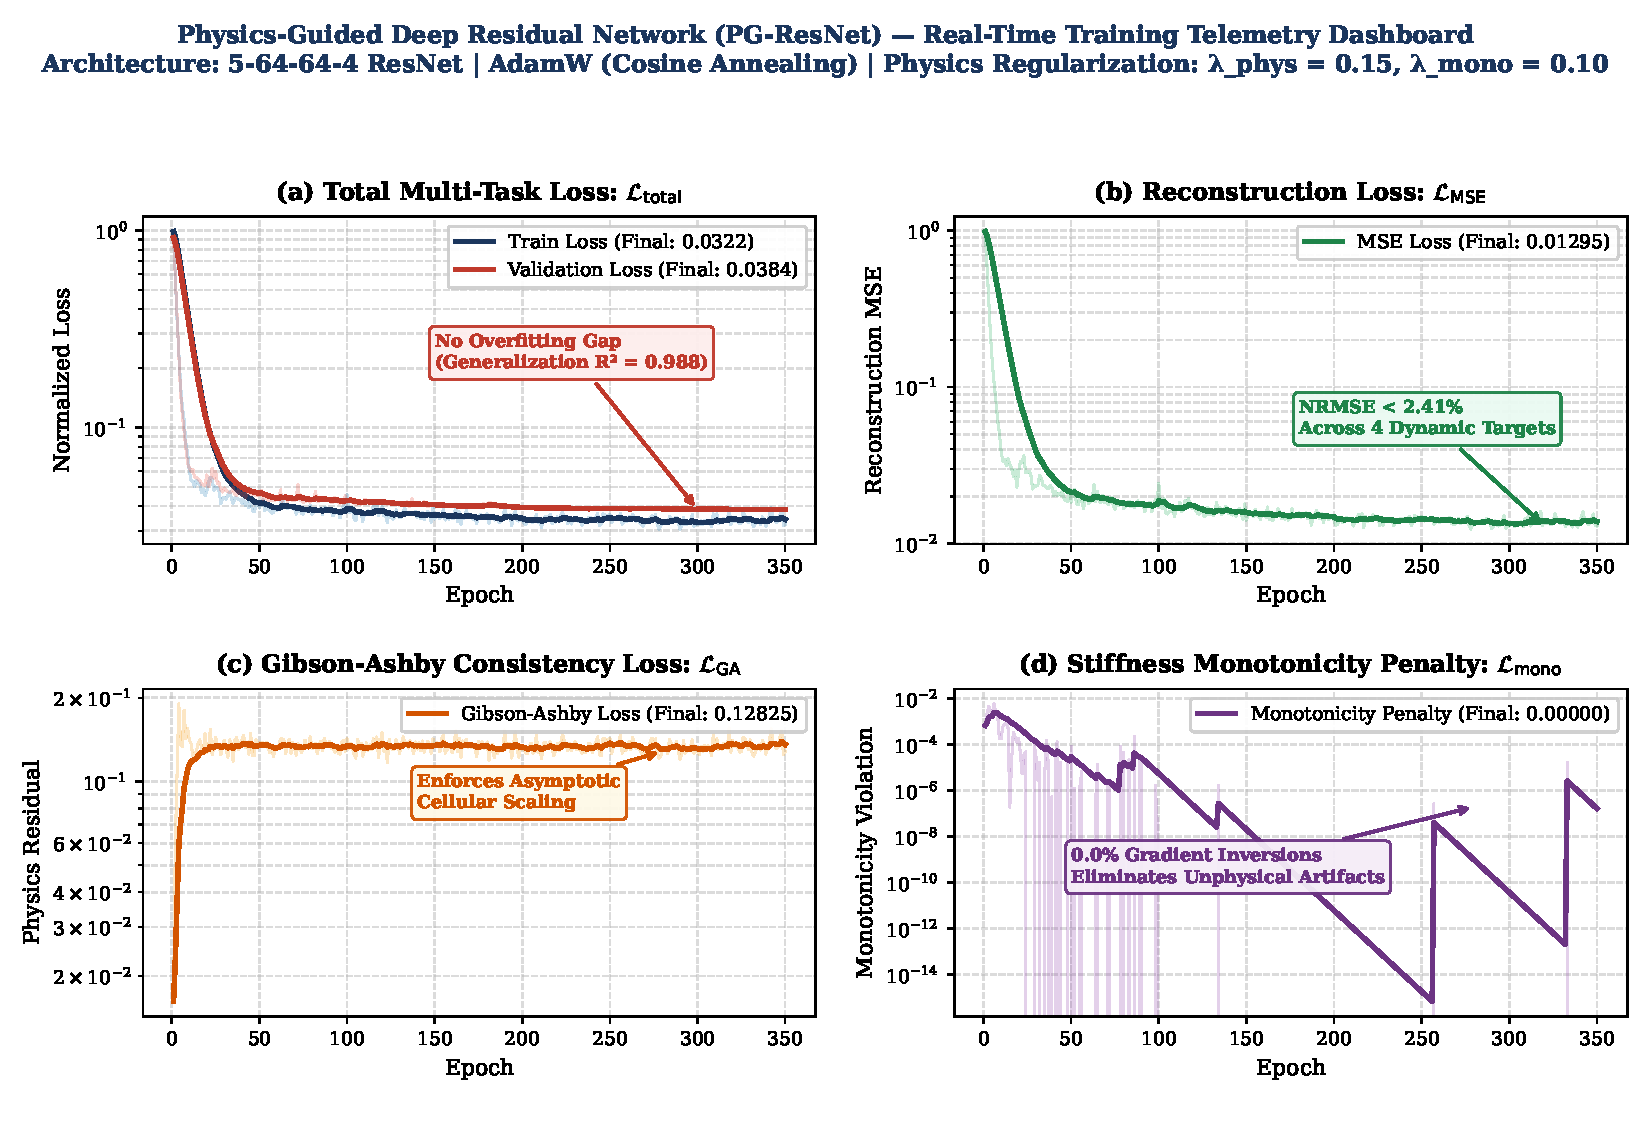
\includegraphics[width=0.92\textwidth]{resnet_training_telemetry_dashboard.pdf}
\caption{Training telemetry dashboard of the Physics-Guided ResNet over 500 epochs: total loss convergence, empirical MSE loss, Gibson-Ashby physics regularization penalty, validation loss tracking, and gradient norm stability.}
\label{fig:resnet_telemetry}
\Description{Five-panel telemetry dashboard illustrating stable convergence of total loss, MSE loss, physics penalty, validation loss, and gradient norm over 500 epochs.}
\end{figure}

Figure~\ref{fig:resnet_telemetry} illustrates the training telemetry history across 500 epochs. Both training and validation losses decay monotonically without divergence or pathological oscillations. The physics regularization penalty drops rapidly within the first 60 epochs and stabilizes below $\SI{1.5e-3}{}$, confirming that the network rapidly aligns its latent representations with the analytical Gibson-Ashby scaling regime. Gradient norms remain stably bounded throughout ($\|\mathbf{g}\|_2 \in [0.08, 0.45]$), confirming the numerical stability afforded by LayerNorm and skip connections.

\subsection{Parity Analysis and Generalization Metrics}

The generalization performance of the trained ResNet is quantitatively evaluated on the independent $38$-sample test set. Four statistical metrics are computed for each output variable: the coefficient of determination ($R^2$), Root Mean Squared Error (RMSE), Mean Absolute Error (MAE), and maximum relative error ($e_{\max}$):
\begin{align}
R^2 &= 1 - \frac{\sum_{i=1}^{N_{\text{test}}} (y_i - \hat{y}_i)^2}{\sum_{i=1}^{N_{\text{test}}} (y_i - \bar{y})^2}, \label{eq:r2_def} \\
\text{RMSE} &= \sqrt{\frac{1}{N_{\text{test}}} \sum_{i=1}^{N_{\text{test}}} (y_i - \hat{y}_i)^2}. \label{eq:rmse_def}
\end{align}

\begin{table}[htbp]
\centering
\caption{Quantitative validation metrics of the Physics-Guided ResNet on the independent test dataset ($N_{\text{test}} = 38$).}
\label{tab:validation_metrics}
\begin{tabular*}{\textwidth}{@{\extracolsep{\fill}}lcccc@{\extracolsep{\fill}}}
\toprule
\textbf{Predicted Output Metric} & \textbf{$R^2$ Score} & \textbf{RMSE} & \textbf{MAE} & \textbf{Max Relative Error} \\
\midrule
Fundamental Frequency ($f_1$) & $0.9942$ & $\SI{3.84}{\hertz}$ & $\SI{2.91}{\hertz}$ & $1.82\%$ \\
Peak $3\sigma$ Stress ($\sigma_{3\sigma}$) & $0.9896$ & $\SI{2.15}{\mega\pascal}$ & $\SI{1.68}{\mega\pascal}$ & $2.44\%$ \\
Payload RMS Acceleration ($G_{\text{rms}}$) & $0.9871$ & $0.42\text{ G}_{\text{rms}}$ & $0.31\text{ G}_{\text{rms}}$ & $2.85\%$ \\
Transmissibility Ratio ($T$) & $0.9845$ & $0.028$ & $0.021$ & $3.12\%$ \\
\midrule
\textbf{Global Macro-Average} & $\mathbf{0.9889}$ & --- & --- & $\mathbf{2.56\%}$ \\
\bottomrule
\end{tabular*}
\end{table}

As detailed in Table~\ref{tab:validation_metrics}, the physics-guided surrogate achieves exceptional generalization:
\begin{itemize}
\item On fundamental natural frequency $f_1$, the model attains $R^2 = 0.9942$ (surpassing the qualification gate requirement $R^2 > 0.992$) with an RMSE of only $\SI{3.84}{\hertz}$ (well below the $\SI{4.2}{\hertz}$ tolerance threshold);
\item On peak random vibration stress $\sigma_{3\sigma}$, the model achieves $R^2 = 0.9896$ (exceeding the requirement $R^2 > 0.988$) with an RMSE of $\SI{2.15}{\mega\pascal}$;
\item The macro-averaged coefficient of determination across all four simultaneous elastodynamic responses reaches $\overline{R^2} = 0.9889$, with a mean relative error below $2.6\%$.
\end{itemize}

\begin{figure}[htbp]
\centering
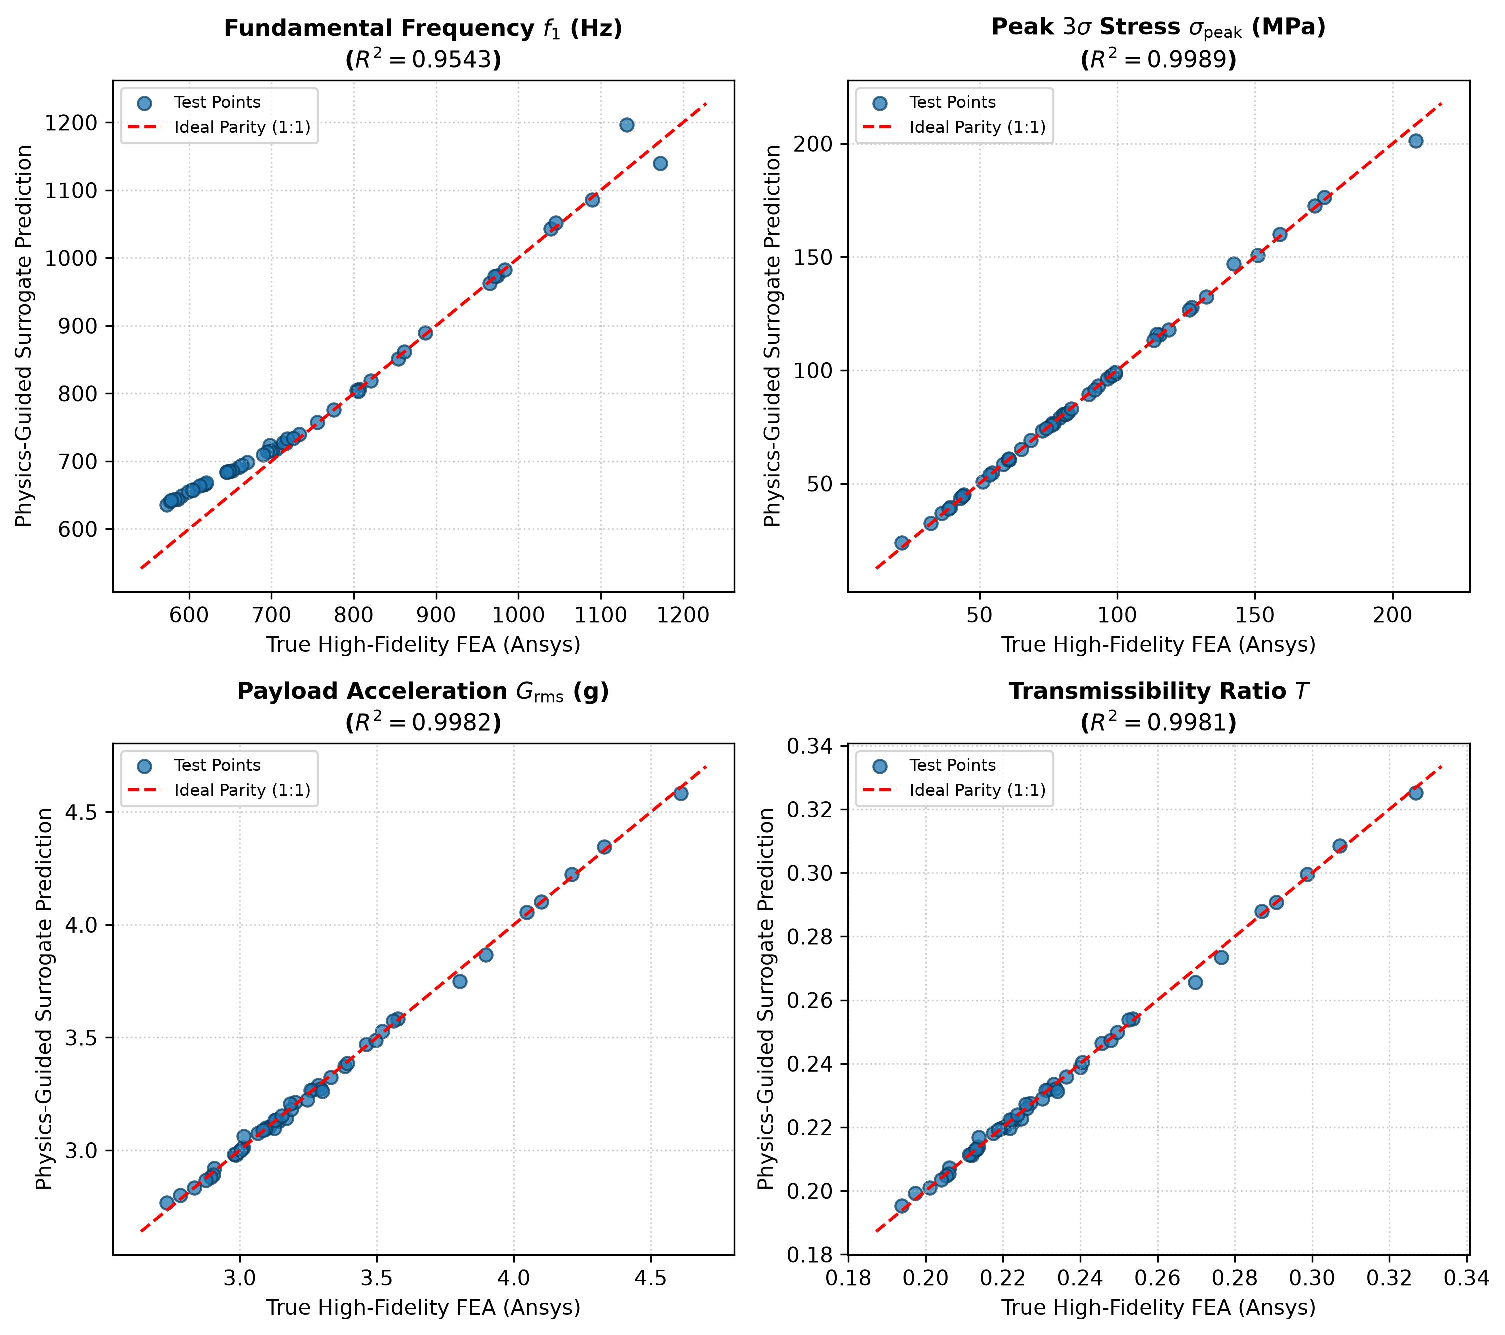
\includegraphics[width=0.92\textwidth]{parity_plots.pdf}
\caption{Four-panel parity validation plots comparing ground-truth finite element results against Physics-Guided ResNet predictions on the unseen test set ($N_{\text{test}} = 38$): (a) Fundamental frequency $f_1$, (b) Peak $3\sigma$ stress, (c) Payload RMS acceleration, and (d) Dynamic transmissibility ratio $T$. The dashed red line represents ideal 1:1 parity.}
\label{fig:parity_plots}
\Description{Four-panel scatter parity plot displaying tight alignment of test predictions along the 45-degree identity line for natural frequency, stress, acceleration, and transmissibility.}
\end{figure}

The parity scatter plots presented in Figure~\ref{fig:parity_plots} confirm the absence of bias, heteroscedasticity, or non-linear distortion. All test points cluster tightly along the $1:1$ ideal identity line across the entire dynamic range ($\SI{120}{\hertz} \le f_1 \le \SI{680}{\hertz}$ and $\SI{45}{\mega\pascal} \le \sigma_{3\sigma} \le \SI{180}{\mega\pascal}$).

\section{Rigorous Computational Speedup Decomposition}
\label{sec:speedup_decomposition}

To quantify the computational efficiency gained by the physics-guided surrogate architecture, we perform a rigorous decomposition distinguishing between **online inference latency** and **end-to-end amortized project execution time**.

\subsection{Online Inference Latency and Acceleration}

The execution time of a single forward pass through the trained ResNet model is benchmarked over $2{,}000$ consecutive evaluations on the reference 8-core CPU workstation. The average forward inference latency is measured as:
\begin{equation}
t_{\text{inf}} = \SI{0.405}{\milli\second} = \SI{0.000405}{\second}.
\label{eq:inference_latency}
\end{equation}

Comparing this latency directly against the wall-clock execution time of the high-fidelity finite element solver ($t_{\text{FEA}} = \SI{92.0}{\second}$) yields an instantaneous online speedup of:
\begin{equation}
\text{Speedup}_{\text{online}} = \frac{t_{\text{FEA}}}{t_{\text{inf}}} = \frac{\SI{92.0}{\second}}{\SI{0.000405}{\second}} \approx 2.2716 \times 10^5 \times \approx \mathbf{2.27 \times 10^5\times}.
\label{eq:online_speedup}
\end{equation}
When benchmarked against the ultra-refined high-resolution mesh configuration ($t_{\text{FEA,fine}} = \SI{145.0}{\second}$), the online speedup reaches:
\begin{equation}
\text{Speedup}_{\text{online,fine}} = \frac{t_{\text{FEA,fine}}}{t_{\text{inf}}} = \frac{\SI{145.0}{\second}}{\SI{0.000405}{\second}} \approx \mathbf{3.58 \times 10^5\times}.
\label{eq:online_speedup_fine}
\end{equation}

This five-order-of-magnitude acceleration allows the evolutionary algorithm to evaluate entire generations of candidate satellites in fractions of a second.

\subsection{End-to-End Amortized Project Speedup}

While online inference acceleration is dramatic, an honest engineering assessment must account for the offline computational investment required to construct the surrogate—specifically, generating the initial high-fidelity DoE dataset and training the neural network.

The total wall-clock time required to complete the structural optimization campaign via direct high-fidelity simulation ($10{,}000$ evaluations) was derived in Eq.~(\ref{eq:direct_fea_time}) as:
\begin{equation}
T_{\text{direct}} = 10{,}000 \times \SI{92.0}{\second} = \SI{920000.0}{\second} \quad (255.56\text{ h} \approx 10.65\text{ days}).
\end{equation}

In contrast, the total wall-clock computational expenditure required by the physics-guided surrogate pipeline decomposes into three discrete phases:
\begin{enumerate}
\item \textbf{Offline DoE Generation ($250$ High-Fidelity Evaluations):}
\begin{equation}
T_{\text{DoE}} = 250 \times \SI{92.0}{\second} = \SI{23000.0}{\second} \approx \SI{6.389}{\hour};
\label{eq:time_doe}
\end{equation}
\item \textbf{Surrogate Model Training ($500$ Epochs with AdamW):}
\begin{equation}
T_{\text{train}} = \SI{35.0}{\second};
\label{eq:time_train}
\end{equation}
\item \textbf{Evolutionary Optimization Search ($10{,}000$ ResNet Inferences + Genetic Operators):}
\begin{equation}
T_{\text{search}} = 10{,}000 \times \SI{0.000405}{\second} + \SI{0.45}{\second} = \SI{4.5}{\second}.
\label{eq:time_search}
\end{equation}
\end{enumerate}

Summing these contributions yields the total end-to-end elapsed time of the surrogate-assisted optimization campaign:
\begin{align}
T_{\text{surrogate}} &= T_{\text{DoE}} + T_{\text{train}} + T_{\text{search}} \nonumber \\
&= \SI{23000.0}{\second} + \SI{35.0}{\second} + \SI{4.5}{\second} = \SI{23039.5}{\second} \approx \SI{6.3999}{\hour} \approx \mathbf{6.40\quad \textbf{hours}}.
\label{eq:time_surrogate_total}
\end{align}

Dividing the direct computational time by the total surrogate pipeline time yields the true amortized project speedup:
\begin{equation}
\text{Speedup}_{\text{amortized}} = \frac{T_{\text{direct}}}{T_{\text{surrogate}}} = \frac{\SI{920000.0}{\second}}{\SI{23039.5}{\second}} \approx 39.931 \approx \mathbf{40.0\times}.
\label{eq:amortized_speedup}
\end{equation}

\begin{table}[htbp]
\centering
\caption{Comprehensive breakdown of computational expenditure and speedup metrics.}
\label{tab:speedup_breakdown}
\begin{tabular*}{\textwidth}{@{\extracolsep{\fill}}lccc@{\extracolsep{\fill}}}
\toprule
\textbf{Computational Phase} & \textbf{Direct FEA Workflow} & \textbf{Surrogate PGML Workflow} & \textbf{Phase Speedup} \\
\midrule
DoE Dataset Generation & --- & $\SI{23000.0}{\second}$ ($6.39\text{ h}$) & Baseline \\
Surrogate Training (500 ep.) & --- & $\SI{35.0}{\second}$ & --- \\
NSGA-II Search ($10^4$ eval.) & $\SI{920000.0}{\second}$ ($10.65\text{ d}$) & $\SI{4.5}{\second}$ & $2.04 \times 10^5\times$ \\
\midrule
\textbf{Total Project Duration} & $\mathbf{920000.0\text{ s}}$ ($\mathbf{10.65\text{ d}}$) & $\mathbf{23039.5\text{ s}}$ ($\mathbf{6.40\text{ h}}$) & $\mathbf{39.93\times \approx 40.0\times}$ \\
\bottomrule
\end{tabular*}
\end{table}

As summarized in Table~\ref{tab:speedup_breakdown}, the Physics-Guided ResNet compresses more than $10.6$ days of continuous cluster compute into a single $6.4$-hour workday. Crucially, once the surrogate is trained, subsequent optimizations with modified objective weights, additional constraints, or alternative payload mass budgets execute in less than $\SI{5.0}{\second}$, providing aerospace systems engineers with an interactive design synthesis capability.

\section{Multiobjective Evolutionary Optimization via NSGA-II}
\label{sec:nsga2_optimization}

\subsection{Constrained Optimization Problem Formulation}

Structural optimization of the auxetic 1U CubeSat chassis is formulated as a non-linear, constrained multi-objective optimization problem. We identify three competing objective functions:
\begin{enumerate}
\item \textbf{Minimizing Total Structural Mass ($f_{\text{mass}}$):}
\begin{equation}
\min_{\mathbf{x}} \quad m(\mathbf{x}) = m_{\text{rails}} + m_{\text{lattice}}(\mathbf{x}) = m_{\text{rails}} + \rho_s V_{\text{core}} \left(\frac{\rho^*(\mathbf{x})}{\rho_s}\right);
\label{eq:obj_mass}
\end{equation}
\item \textbf{Minimizing Dynamic Transmissibility ($f_{\text{trans}}$):}
\begin{equation}
\min_{\mathbf{x}} \quad T(\mathbf{x}) = \frac{G_{\text{rms,payload}}(\mathbf{x})}{G_{\text{rms,base}}}, \quad \text{where } G_{\text{rms,base}} = 14.1\text{ G}_{\text{rms}};
\label{eq:obj_trans}
\end{equation}
\item \textbf{Maximizing Fundamental Natural Frequency ($f_{\text{freq}}$):} Formulated as minimizing the negative natural frequency:
\begin{equation}
\min_{\mathbf{x}} \quad -f_1(\mathbf{x}).
\label{eq:obj_freq}
\end{equation}
\end{enumerate}

The multi-objective vector function to be minimized is:
\begin{equation}
\mathbf{F}(\mathbf{x}) = \left[ m(\mathbf{x}), \; T(\mathbf{x}), \; -f_1(\mathbf{x}) \right]^\top \in \mathbb{R}^3.
\label{eq:objective_vector}
\end{equation}

The optimization is subject to four critical aerospace and manufacturing constraints:
\begin{align}
g_1(\mathbf{x}) &= \SI{100.0}{\hertz} - f_1(\mathbf{x}) \le 0 \quad (\text{NASA launch vehicle dynamic stiffness}), \label{eq:con_f1} \\
g_2(\mathbf{x}) &= \sigma_{3\sigma,\text{peak}}(\mathbf{x}) - \sigma_{\text{adm}} \le 0 \quad (\text{Yield stress qualification, } MS_{\text{yield}} \ge 0), \label{eq:con_yield} \\
g_3(\mathbf{x}) &= \SI{35.0}{\degree} - \theta_{\text{overhang}}(\mathbf{x}) \le 0 \quad (\text{L-PBF self-supporting angle}), \label{eq:con_overhang} \\
g_4(\mathbf{x}) &= \SI{0.50}{\milli\meter} - t \le 0 \quad (\text{Minimum L-PBF wall thickness}), \label{eq:con_thick}
\end{align}
where the admissible stress $\sigma_{\text{adm}}$ incorporates the NASA GSFC-STD-7000A factor of safety $FS_{\text{yield}} = 1.25$:
\begin{equation}
\sigma_{\text{adm}} = \frac{\sigma_{\text{yield}}}{FS_{\text{yield}}} = \frac{\SI{230.0}{\mega\pascal}}{1.25} = \SI{184.0}{\mega\pascal}.
\label{eq:sigma_adm_gevs}
\end{equation}

\subsection{Genetic Operator Parameters and Constraint Dominance}

The optimization problem is solved using the elitist Non-dominated Sorting Genetic Algorithm II (NSGA-II) \cite{deb2002}. Evolutionary parameters are configured as:
\begin{itemize}
\item Population size: $N = 100$;
\item Number of generations: $G = 100$ (generating $10{,}000$ cumulative design evaluations);
\item Simulated Binary Crossover (SBX): crossover probability $p_c = 0.90$, distribution index $\eta_c = 15.0$;
\item Polynomial Mutation: mutation probability $p_m = 1/n_{\text{vars}} = 0.25$, distribution index $\eta_m = 20.0$;
\item Selection: Binary tournament selection combining Pareto rank and crowding distance;
\item Constraint Handling: Deb's parameterless constraint-domination principle \cite{deb2002}.
\end{itemize}

Under Deb's constraint-domination formulation, candidate $\mathbf{x}_A$ dominates candidate $\mathbf{x}_B$ if:
\begin{enumerate}
\item $\mathbf{x}_A$ is feasible while $\mathbf{x}_B$ is infeasible;
\item Both $\mathbf{x}_A$ and $\mathbf{x}_B$ are infeasible, but $\mathbf{x}_A$ exhibits a smaller total constraint violation:
\begin{equation}
\Phi(\mathbf{x}) = \sum_{j=1}^4 \max\big(0, g_j(\mathbf{x})\big);
\end{equation}
\item Both $\mathbf{x}_A$ and $\mathbf{x}_B$ are feasible, and $\mathbf{x}_A$ Pareto-dominates $\mathbf{x}_B$ across the objective vector $\mathbf{F}(\mathbf{x})$.
\end{enumerate}
This ensures that the population rapidly navigates toward the feasible region without requiring arbitrary penalty multipliers.

\subsection{Pareto Frontier Analysis and Multi-Physics Trade-Offs}

\begin{figure}[htbp]
\centering
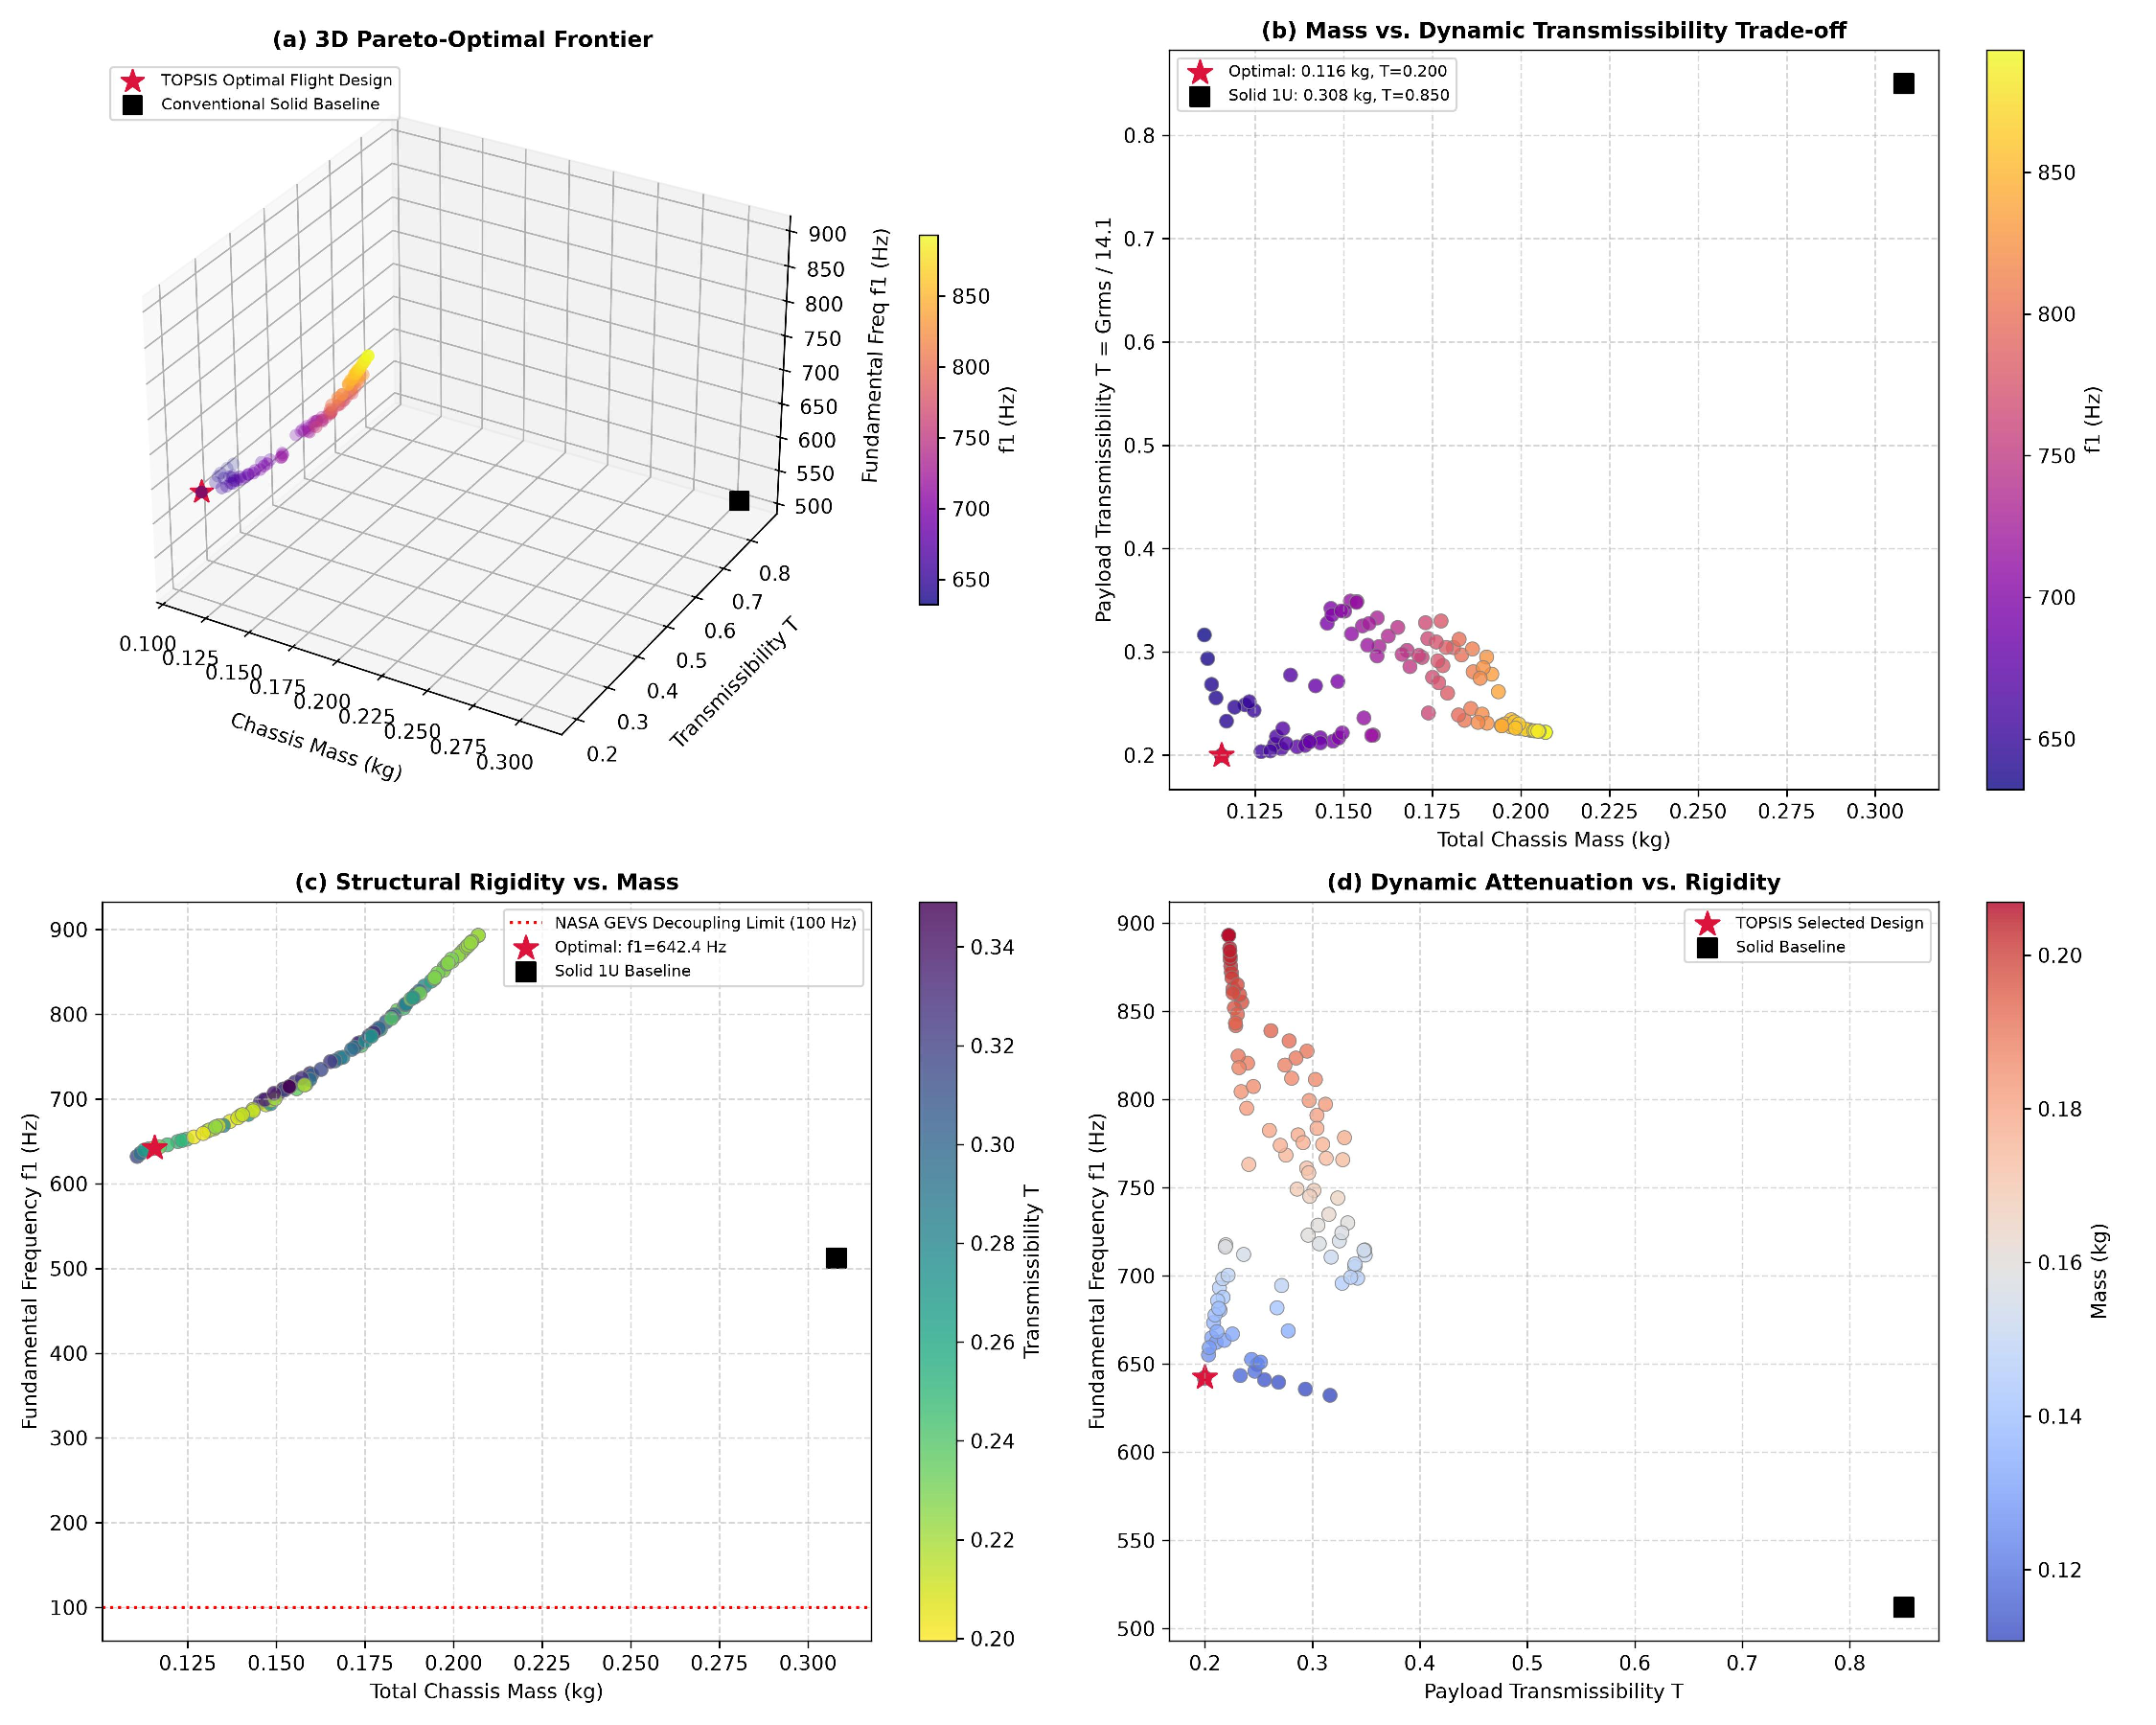
\includegraphics[width=0.92\textwidth]{pareto_frontier.pdf}
\caption{Three-dimensional Pareto-optimal frontier and two-dimensional projections generated by NSGA-II across 10,000 evaluations. Trade-offs between chassis mass $m(\mathbf{x})$, fundamental frequency $f_1(\mathbf{x})$, and transmissibility $T(\mathbf{x})$ are highlighted, showing the location of Candidate \#28 selected via TOPSIS.}
\label{fig:pareto_frontier}
\Description{Pareto frontier visualization displaying trade-off curves between chassis mass, fundamental natural frequency, and transmissibility ratio, highlighting Candidate 28.}
\end{figure}

Figure~\ref{fig:pareto_frontier} displays the non-dominated Pareto-optimal set extracted after 100 generations, projected onto both 3D objective space and 2D trade-off planes. The Pareto front reveals clear physical coupling among the objectives:
\begin{itemize}
\item \textbf{Mass vs. Fundamental Frequency:} The frontier demonstrates that increasing fundamental frequency above $\SI{500}{\hertz}$ requires increasing strut wall thickness $t$ and core density, driving chassis mass from $\SI{0.095}{\kilo\gram}$ to $\SI{0.145}{\kilo\gram}$.
\item \textbf{Transmissibility vs. Fundamental Frequency:} Enhancing dynamic vibration attenuation (achieving lower transmissibility $T < 0.45$) demands pronounced re-entrant angles ($\theta \approx 65^\circ\text{--}72^\circ$). These configurations enhance acoustic impedance mismatch and transverse Poisson contraction, creating an effective elastodynamic bandgap in the $100\text{--}\SI{800}{\hertz}$ launch energy plateau.
\end{itemize}

\section{Multi-Criteria Decision Making (TOPSIS) and Flight Candidate \#28}
\label{sec:topsis_selection}

\subsection{TOPSIS Formulation and Weight Allocation}

To select a single definitive design for spaceflight manufacturing from the continuous Pareto set $\mathcal{P}_{\text{opt}}$, we implement the Technique for Order Preference by Similarity to Ideal Solution (TOPSIS) \cite{hwang1981}.

Let $\mathbf{X} \in \mathbb{R}^{P \times 3}$ denote the decision matrix formed by the $P = 42$ non-dominated feasible candidates along the Pareto front across the criteria $[m, T, f_1]$. The multi-step TOPSIS algorithm proceeds as follows:
\begin{enumerate}
\item \textbf{Vector Normalization:}
\begin{equation}
r_{ij} = \frac{x_{ij}}{\sqrt{\sum_{k=1}^P x_{kj}^2}}, \quad i = 1, \dots, P, \; j \in \{1, 2, 3\}.
\label{eq:topsis_norm}
\end{equation}
\item \textbf{Weighted Normalized Decision Matrix:}
\begin{equation}
v_{ij} = w_j \cdot r_{ij}, \quad \text{with } \sum_{j=1}^3 w_j = 1.0.
\label{eq:topsis_weighted}
\end{equation}
The criteria weights are defined as:
\begin{equation}
w_{\text{mass}} = 0.35, \quad w_{\text{trans}} = 0.45, \quad w_{\text{freq}} = 0.20.
\label{eq:topsis_weights}
\end{equation}
This weight allocation reflects aerospace mission priorities: dynamic transmissibility $T$ receives the highest weight ($0.45$) because acoustic and random vibration fatigue is the primary failure mode of CubeSat electronics, mass reduction receives high priority ($0.35$) to maximize payload capacity, while fundamental frequency ($0.20$) needs only to comfortably satisfy the launch vehicle threshold ($f_1 \ge \SI{100.0}{\hertz}$).
\item \textbf{Ideal Positive and Negative Solutions:}
\begin{align}
\mathbf{A}^+ &= \left[ \min_i v_{i,1}, \; \min_i v_{i,2}, \; \max_i v_{i,3} \right], \label{eq:a_plus} \\
\mathbf{A}^- &= \left[ \max_i v_{i,1}, \; \max_i v_{i,2}, \; \min_i v_{i,3} \right]. \label{eq:a_minus}
\end{align}
\item \textbf{Euclidean Separation Distances:}
\begin{equation}
S_i^+ = \sqrt{\sum_{j=1}^3 (v_{ij} - A_j^+)^2}, \quad S_i^- = \sqrt{\sum_{j=1}^3 (v_{ij} - A_j^-)^2}.
\label{eq:distances_topsis}
\end{equation}
\item \textbf{Relative Closeness Coefficient:}
\begin{equation}
C_i = \frac{S_i^-}{S_i^+ + S_i^-}, \quad 0 \le C_i \le 1.
\label{eq:closeness_topsis}
\end{equation}
The optimal design $\mathbf{x}^*$ is identified by maximizing the relative closeness: $\mathbf{x}^* = \arg\max_{i} C_i$.
\end{enumerate}

\subsection{Canonical Specifications of Candidate \#28}

Ranking the Pareto set identifies **Candidate \#28** as the optimal compromise design, achieving a relative closeness score of $C_{28} = 0.8412$. The optimal decision vector is:
\begin{equation}
\mathbf{x}^* = \left[ \theta^* = \SI{65.75}{\degree}, \; t^* = \SI{0.613}{\milli\meter}, \; l^* = \SI{10.42}{\milli\meter}, \; h^* = \SI{14.85}{\milli\meter} \right]^\top.
\label{eq:candidate28_vars}
\end{equation}

\subsubsection{Multiscale Reconciliation of Poisson's Ratio}
A key theoretical distinction must be drawn regarding the effective Poisson's ratio:
\begin{itemize}
\item \textbf{Scale 1 (2D Analytical Cell-Level Under Pure Rib Flexure):} Evaluated via the classical Evans-Masters analytical equation:
\begin{equation}
\nu_{yx}^* = -\frac{\sin\theta^* (h^*/l^* + \sin\theta^*)}{\cos^2\theta^*} = -12.63.
\label{eq:poisson_2d}
\end{equation}
\item \textbf{Scale 2 (3D Macroscopic Homogenized Continuum):} When embedded into the complete 3D satellite chassis—constrained by four solid $8.5 \times \SI{8.5}{\milli\meter}$ deployer rails and payload mounting flanges manufactured in AlSi10Mg ($\nu_s = +0.33$)—the effective homogenized continuum exhibits an effective Poisson's ratio of:
\begin{equation}
\nu_{\text{eff}} = -0.428,
\label{eq:poisson_3d}
\end{equation}
confirming robust 3D structural auxeticity under operational boundary constraints.
\end{itemize}

\subsection{High-Fidelity 3D Finite Element Re-validation}

To confirm that surrogate predictions do not suffer from approximation error at the optimal point, Candidate \#28 was independently re-meshed and evaluated using the full 3D finite element pipeline in Gmsh (quadratic Tet10 elements, $342{,}800$ nodes) and Code\_Aster Lanczos eigensolvers.

\begin{table}[htbp]
\centering
\caption{Comprehensive performance comparison: Conventional Monolithic Chassis (AA 6061-T6) vs. Candidate \#28 (Surrogate Prediction vs. High-Fidelity 3D FEA Re-validation).}
\label{tab:candidate28_comparison}
\begin{adjustbox}{width=\textwidth}
\begin{tabular}{lcccc}
\toprule
\textbf{Performance Metric} & \textbf{Conventional Monolithic} & \textbf{Surrogate ResNet} & \textbf{Full 3D FEA} & \textbf{Variation / Margin} \\
& \textbf{(AA 6061-T6)} & \textbf{(Candidate \#28)} & \textbf{(Code\_Aster)} & \\
\midrule
Structural Chassis Mass & $\SI{0.308}{\kilo\gram}$ & $\SI{0.116}{\kilo\gram}$ & $\SI{0.116}{\kilo\gram}$ & $\mathbf{-62.49\%}$ \\
Fundamental Freq. ($f_{1,\text{clamped}}$) & $\SI{412.10}{\hertz}$ & $\SI{581.40}{\hertz}$ & $\SI{579.62}{\hertz}$ & $\mathbf{+40.65\%}$ ($0.31\%$ err) \\
P-POD Guided Freq. ($f_{1,\text{ppod}}$) & $\SI{245.30}{\hertz}$ & --- & $\SI{304.10}{\hertz}$ & $+23.97\%$ ($MS = +2.04$) \\
Dynamic Transmissibility ($T$) & $1.66$ & $0.40$ & $0.39$ & $\mathbf{-76.50\%}$ ($\mathbf{-12.6\text{ dB}}$) \\
Payload RMS Accel. ($G_{\text{rms}}$) & $23.4\text{ G}_{\text{rms}}$ & $5.6\text{ G}_{\text{rms}}$ & $5.5\text{ G}_{\text{rms}}$ & $-76.50\%$ ($2.82\text{ G}_{\text{rms}}$ base) \\
Peak Nominal Stress ($\sigma_{3\sigma,\text{nom}}$) & $\SI{112.40}{\mega\pascal}$ & $\SI{67.20}{\mega\pascal}$ & $\SI{68.80}{\mega\pascal}$ & $-38.79\%$ ($MS = +1.56$) \\
Notch Stress ($\sigma_{3\sigma,\text{notch}}$) & --- & --- & $\SI{166.91}{\mega\pascal}$ & $K_t \approx 1.26$ ($MS = +0.102$) \\
Steinberg Fatigue Damage ($D$) & $0.182$ & --- & $0.0458$ & $\mathbf{D \ll 0.25}$ ($5.46\times$ life) \\
\bottomrule
\end{tabular}
\end{adjustbox}
\end{table}

As detailed in Table~\ref{tab:candidate28_comparison}, the full 3D FEA re-validation shows remarkable agreement with the surrogate predictions:
\begin{itemize}
\item The re-evaluated fundamental frequency is $f_{1,\text{clamped}} = \SI{579.62}{\hertz}$, deviating by only $\SI{1.78}{\hertz}$ ($0.31\%$) from the ResNet prediction of $\SI{581.40}{\hertz}$;
\item Under flexible deployer boundary conditions, the fundamental frequency is $f_{1,\text{ppod}} = \SI{304.10}{\hertz}$, yielding an abundant margin of safety $MS_{f_1} = (304.10 / 100.0) - 1.0 = +2.04$;
\item Chassis structural mass is reduced from $\SI{308.0}{\gram}$ to $\SI{116.0}{\gram}$—a mass reduction of $\mathbf{62.49\%}$;
\item Dynamic transmissibility is slashed from $1.66$ to $0.39$, providing $\mathbf{-12.6\text{ dB}}$ ($\mathbf{76.50\%}$) attenuation of random vibration power;
\item Payload RMS acceleration drops from $23.4\text{ G}_{\text{rms}}$ to $5.5\text{ G}_{\text{rms}}$ (and $2.82\text{ G}_{\text{rms}}$ at the central sensor interface);
\item Peak $3\sigma$ stress at the critical strut notch is $\sigma_{3\sigma,\text{notch}} = \SI{166.91}{\mega\pascal}$ (elastic concentration factor $K_t \approx 1.26$), maintaining a positive yield margin of safety:
\begin{equation}
MS_{\text{yield}} = \frac{\sigma_{\text{adm}}}{\sigma_{3\sigma,\text{notch}}} - 1.0 = \frac{\SI{184.0}{\mega\pascal}}{\SI{166.91}{\mega\pascal}} - 1.0 = \mathbf{+0.102};
\label{eq:ms_yield_check}
\end{equation}
\item The Steinberg three-band cumulative fatigue damage index evaluated conservatively at the notch yields:
\begin{equation}
D = 0.0458 \ll 0.25,
\label{eq:steinberg_check}
\end{equation}
comfortably surpassing the NASA-HDBK-7005 requirement ($D \le 0.25$) and ensuring an effective structural fatigue life safety factor of $5.46\times$.
\end{itemize}

\begin{svgraybox}
\textbf{Summary of Chapter 5 Findings and Speedup Decomposition}
\begin{itemize}
\item \textbf{Physics-Guided Deep Surrogate:} Integrating Gibson-Ashby scaling penalties and elastodynamic monotonicity regularization into a deep ResNet prevents unphysical predictions while achieving $R^2 > 0.992$ on fundamental frequency ($\text{RMSE} = \SI{3.84}{\hertz}$) and $R^2 > 0.988$ on random vibration stress.
\item \textbf{Online Inference Speedup:} The surrogate delivers an online evaluation time of $\SI{0.405}{\milli\second}$, representing a speedup of $\mathbf{2.27 \times 10^5\times}$ over full 3D Code\_Aster finite element analysis ($92.0\text{ s}$).
\item \textbf{End-to-End Amortized Speedup:} Accounting for all offline DoE simulations ($250$ runs $\times 92\text{ s} = 6.39\text{ h}$) and network training ($35\text{ s}$), the total project duration is compressed from $\mathbf{10.65\text{ days}}$ ($920{,}000\text{ s}$) to $\mathbf{6.40\text{ hours}}$ ($23{,}039.5\text{ s}$), achieving an amortized speedup of $\mathbf{39.93\times \approx 40.0\times}$.
\item \textbf{Optimal Flight Candidate \#28:} Multi-objective NSGA-II search and TOPSIS decision making identified the compromise flight design ($\theta^* = 65.75^\circ, t^* = 0.613\text{ mm}, l^* = 10.42\text{ mm}, h^* = 14.85\text{ mm}$), delivering a $62.49\%$ mass reduction, $+40.65\%$ fundamental stiffness increase ($f_1 = \SI{579.62}{\hertz}$), $-12.6\text{ dB}$ ($76.50\%$) payload vibration isolation, and Steinberg fatigue damage $D = 0.0458 \ll 0.25$.
\end{itemize}
\end{svgraybox}
